\documentclass{article}
\usepackage[utf8]{inputenc}
\usepackage{titlesec}
\usepackage{natbib}
\usepackage{graphicx}
\graphicspath{ {img/} }
\usepackage{amsmath}
\allowdisplaybreaks[1]
\usepackage{amsfonts}
\usepackage{enumitem}
\usepackage{bbm}
\usepackage{bm}
\usepackage{float}
\usepackage{titlesec}
\usepackage{parskip}
\usepackage{mathtools}
\setcounter{section}{0}
\usepackage[font={small ,it}]{caption}
\usepackage[a4paper, total={6in, 8in}]{geometry}
\usepackage{xcolor}
\usepackage{bbm}
\usepackage{subcaption}
\usepackage{listings}

\def\SPSB#1#2{\rlap{\textsuperscript{\textcolor{black}{#1}}}\SB{#2}}
\def\SP#1{\textsuperscript{\textcolor{black}{#1}}}
\def\SB#1{\textsubscript{\textcolor{black}{#1}}}
\DeclareMathOperator*{\argmax}{arg\,max}  % in your preamble
\newcommand\iid{i.i.d.}
\newcommand\pN{\mathcal{N}}

\begin{document}

\newcommand{\vect}[1]{\boldsymbol{#1}}
\begin{titlepage}

    \begin{center}
       \vspace*{1cm}
        
        \Huge
        \textbf{Gaussian Mixture Model on Eyes data}
        
        \vspace{0.5cm}
        \LARGE
        \textbf{Computational Statistics}
        
        \vspace{1.5cm}
        
        \textbf{Simone Totaro}
        
        \vfill
        
        July 2017
        
        \vspace{0.8cm}
    
    \end{center}
\end{titlepage}
\section{Introduction}
The aim of this project is to build a complete Bayesian analysis for 48 measurements of peak of sensitivity wrt the wavelengths of microspectrophotometric records Bowmaker et al. (1985), coming from a single monkey. The outcome of the Bayesian analysis is to provide a possible model that explains the measurements, as well as the parameters underlying the phenomena. This is a known example for Wingbugs practitioners and it has been reviewed from Diebolt and Robert (1994). The proposed model is a mixture of Gaussian distribution, with conjugate priors that are appropriately specified below. The project is organized as follows:

In Model Specification we review the linear mixture model with Gaussian distribution with some of its modelling properties and shortcomings, using a toy example to guide our understanding of the analysis. Then we turn in analyzing the data of the 48 measurements of the monkeys, and we finally use a Gibbs Sampling algorithm as the inference tool for the proposed task. We conclude the project by discussing the difference in results obtained wrt JAGS model confronting point estimates, interval estimates and model selection criterion such as DIC and posterior predictive check.


\section{Model specification}
The Gaussian Mixture model is a particular case of a broader family of the finite mixture models. In general, suppose we have C components, each of them representing the particular information contained in C groups. Each group is described with it's distribution $f_c(\cdot \mid \theta)$, also referred as mixture component. The distribution of the overall population is represented as the linear combination of the weighted contribution of each mixture component. Namely, let $w_c$ with $c = {1, C}$ be the weight associated with the mixture of the cth component such that $\sum_{c = 1}^{C} w_c = 1$ and $w_c \geq 0  \ \forall c  \in {1,C}$, then the finite mixture distribution is given by:
\begin{equation}
f(x|\vect \theta) = \sum_{c = 1}^C w_c f_c(x \mid \vect \theta)
\end{equation}

Where $\vect w = (w_1,\cdots , w_c)$ is the vector of weights taking values in the C-1 Simplex. A simplification of this model is such that $f_c$ are part of the same family of distribution, such that $f_c (\cdot \mid \theta_c) = f( \cdot \mid \theta) \in  F = \{f(\cdot \mid \theta), \theta \in \Theta \}$. For our purpose, please consider each mixture component being a Normal distribution with $N(\mu_c, \tau)$ where $\mu$ is the location and $\tau$ is the precision, i.e. $\tau = \sigma^{1/2}$. Thus the parameter is made of 3C - 1 parameters as  $\vect \theta = (\w_c \mu_c, \tau), \ \forall c \in {1,C}$. The population distribution is given by
\begin{equation}
X \mid \vect \theta \sim f(x \mid \theta)  = \sum_{c = 1}^C w_c N(x \mid \mu_c \mid \tau_c)
\end{equation}

\begin{figure}[h!]
    \begin{subfigure}{0.5\textwidth}
        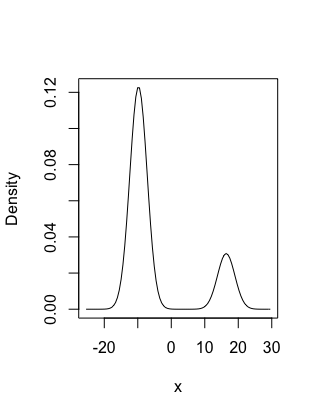
\includegraphics[width=.7\textwidth]{Mix_gauss.png}
        \caption{Mixture of Gaussian with C=2 and shared $\tau$}
        \label{Mixture of gaussians}
    \end{subfigure}
    \begin{subfigure}{0.5\textwidth}
        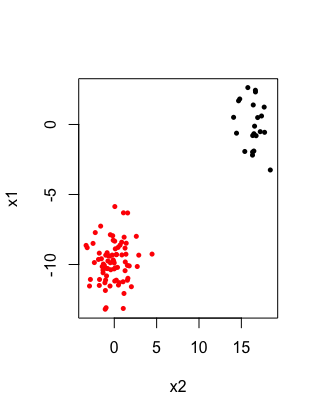
\includegraphics[width=.7\textwidth]{Mix_gauss_2.png}
        \caption{Sample from Mixture of Gaussian}
        \label{Mixture of gaussians}
    \end{subfigure}
\end{figure}


Another way to represent the population distribution is by assuming a latent variable $Z$ which define the presence of the cth component according to its weights. More formally let, $z_{ic}$ be the indicator function of the ith unit in the cth such as $I_{i \in c}(z) \forall \c in \{1, C\}$. $Z | \vect \theta \sim Multinom (1, \vect \w)$. Which allow us to define the $P(z_{ic} = 1 \mid \vect \theta) = w_c$ and $f(x_i \mid \vect \theta, \vect Z_i) \sim \prod_{c=1}^C N(x_i \mid \mu_c \tau_c )^{z_{ic}}$

Suppose we have a sample of i.i.d. $\vect X = (X_1, \cdots , X_n)$ data from the population, the likelihood function can be derived as follow:
\begin{equation}
\begin{split}
L(\vect \theta) &= \prod_{i=1}^n  \sum_{c=1}^C f(x_i \mid \vect\theta) P(z_{ic} = 1 \mid \vect \theta ) \\
&= \prod_{i=1}^n \sum_{c=1}^C N(x_i \mid \mu_c, \tau) P(z_{ix} = 1 \mid \w_{c})
\end{split}
\end{equation}

The log likelihood is given by:
\begin{equation}
\log L(\vect \theta)  = \sum_{i=1}^n \log \sum_{c=1}^C N(x_i \mid \mu_c, \tau) \w_{c}
\end{equation}

Altought the likelihood is straightforward to derive, the summation inside the logarithm make the maximization problem for at least two reasons:
\begin{itemize}
\item the objective function is not convex, in fact we can not guarantee that $\frac{\partial^2 l}{\partial^2 x} > 0 \ \forall x$
\item since the likelihood is invariant to summation and products, we have $C^n$ possible modes which makes hard for standard approximation procedure like EM to find the global maxima.
\end{itemize}

\begin{figure}[h!]
    \centering
    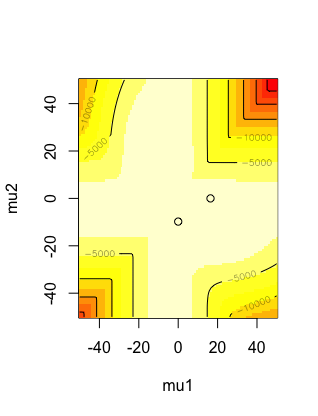
\includegraphics[width=.5\textwidth]{Mix_gauss_3.png}
    \caption{Contour plot of the Observed data likelihood}
    \label{Mixture of gaussians}
\end{figure}

A nicer representation of $l L(\vet \theta)$ can be derived using the completion technique.
% not sure if this is correct
\theoremstyle{definition}
\begin{definition}{Completion}
Let $f(x | \theta)$ be a conditional distribution from the joint distribution $J(\theta, x)$, then $g(\theta)$ is a completion for $f(x |\theta)$ if $\f(x|\theta) \g(\theta) = J(\theta,x)$
\end{definition}
For our purposes, consider the joint distribution of the observed variable and the latent variable, conditionally on the parameter vector $J(x, z \mid \vect\theta)$, according to the previous definition, we can say that $Z$ is a completion for $f(x \mid \vect \theta)$ and we can augment the likelihood making the latent variable explicit in the model formulation. This strategy is also called data augmentation. More formally, let $L_c(\theta, z)$ such as:
\begin{equation}
\begin{split}
L_c(\theta, z) &= \prod_{i=1}^n f(x_i, z_i \mid \vect \theta)) \\
&= \prod_{i=1}^n f(x_i \mid  \vect Z_i, \vect \mu, \vect \tau, \vect w) P(\vect Z_i = z_i \mid \vect \mu, \vect \tau, \vect w) \\
&= \prod_{i=1}^n \prod_{c=1}^C N(x_i | \mu_c \tau_c)^{z_{ic}} \prod_{c=1}^C w_c^{z_{ic}} \\
&= \prod_{i=1}^n \prod_{c=1}^C \Bigg( N(x_1 | \mu_c \tau_c) w_c \Bigg)^{z_{ic}}
\end{split}
\end{equation}

And the log data likelihood is given by:
\begin{equation}
\log L(\vect \theta, \vect z) = \sum_{i=1}^n \sum_{c=1}^C z_{ic}\Bigg (\log w_c + \log N(x_i \mid \mu_c, \tau_c) \Bigg)
\end{equation}

\subsection{Model specification}
Given the previous consideration on the maximization of likelihood function, our approach is to use an MCMC method to obtain a sample of the posterior distribution of the $\vect \theta$. One way is to use conjugate priors on the parameters, in order to obtain full conditional distribution that are simple to compute and code in R. Please remember that choosing priors, i.e. expressing prior belief about a phenomena, for computational reason is statistically meaningful and it's done only for the project purpose.  Remember that the parameter vector is given by $\vect \theta = (\vect \mu, \vect \tau, \vect w)$, thus the prior distribution $\pi(\vect \theta)$ can be defined as:

\begin{equation}
\pi(\vect \theta) = \prod_{c=1}^C \pi(\mu_c) \pi(\tau) \pi(\vect w)  
\end{equation}

Following the previous equation, notice that we assume independence among all the parameters in $\theta$, but only $\mu$ is also \iid from the same prior, while only assume that the mixture weights $\vect w$ are identically distributed, but not independent.

Thus for our scenario we would like to use the following priors:
\begin{align*} 
\pi(\mu) \iid \sim \pN(\mu_0, \tau_0) \\
\pi(\tau) \iid \sim \pGamma(a_0,b_0) \\
\pi(\z) \sim \pDirichlet (1, \vect \alpha)\\
\end{align*}

% The full conditional distribution are straightforward to derive, and as general principle we apply $\pi(\vect \theta, z \mid x) \propto \pi $

% complete data likelihood
% bayesian perspective
% conditional distribution
% results

For the purpose of the exercise, lacking of prior expertise and domain knowledge I have no prior information to impose on the model, nor in the order of the different modes. For this reason I choose to use very diffuse priors, except for the the Dirichlet distribution. This is because by forcing strong prior information on the weight, I except to reduce the number mixed samples from the parameter space.  With this parametrization we still suffer of the label switching problem, and we will have on the posterior sample maybe using the pivot method to re-label each sample. This approach has the advantage of not imposing any constraint on the parameter space, and the exploration performed by the sampler, letting the statistician free to work with diffuse prior belief as in this case. The prior parameters are the following:

\begin{itemize}
\item $\mu_0 = 0, \tau_0 = 1e-6$
\item $a_0 = 1-e3, b_0 = 1-e3$
\item $\vect\alpha = (4,4)$
\end{itemize}


\begin{figure}[h!]
    \begin{subfigure}{0.5\textwidth}
        \includegraphics[width=.7\textwidth]{Mix_gauss_4.png}
        \caption{Traceplot from the Gibbs sampling $\tau$}
        \label{Mixture of gaussians}
    \end{subfigure}
    \begin{subfigure}{0.5\textwidth}
        \includegraphics[width=.7\textwidth]{Mix_gauss_4.png}
        \caption{Posterior distribution of each parameter}
        \label{Mixture of gaussians}
    \end{subfigure}
\end{figure}

In this example we can see the effect of label switching by looking at the Traceplot of the $w_1$, in fact between the 3.000 and 4.000 iteration the chain starts exploring a subspace which doesn't seem consistent with the rest of the chain. It follows that if we use this sample to make inference, the inference itself will be spoiled by transition between modes. In order to resolve the label switching problem, we can rely on the Pivotal Reordering Algorithm introduced by Marin et al (2005). The idea is to use suitable initialization of the chain to use as pivot points to reassign the proper sample to each distribution, by minimizing the Euclidean distance between the suitable initialization and each sample, for each parameter in the $\vect \theta$. This procedure is well implemented in R, in the ```label.switching``` package. 
% explain better how does ti work, a read the paper !

Suitable initialization points to use as pivot points are the MLE estimates of the parameters that can be obtained via the ```MCclust``` package that use the EM algorithm to find the maximum likelihood estimate. With this in mind we can reinizialze the chain and compare the results with the previous run:

% add table here showing the difference between the two runs

As a quick summary, we are going to fit a finite Gaussian mixture model, with diffuse conjugate priors, except for the mixing order, and apply the PRA algorithm to perform relabeling of the sample. By performing this analysis we don't perform any assumption on order of the parameter space, since we have no prior information on how and why they should be split. This approach is different from the one suggest by Robert et al (1998), which impose an order among the means of the model. Moreover, in our case we relax the assumption of single variance for the same mean vector, because we may want to take into account that reaction could be delayed between measurements and variation between pigment reaction could simply be independent. % check the date. 
This intuition is supported by the BIC criterion provided by the `MC clust package`. % add BIC table here


\section{Data}
 


\section{Simulation}
\subsection{Overview}
\subsection{Point estimates}
\subsection{Interval estimates}
\subsection{Model selection}
\end{document}